\documentclass{article}

\usepackage{epsfig,graphics,psfrag,color,rotating}
\usepackage{amsmath,amsfonts,amssymb,bbm}


\textwidth=30cm

\def\X{\mathcal{X}}
\def\un{\mathbbm{1}}
\def\u{\mathrm{u}}

\sloppy


\begin{document}
\thispagestyle{empty}

\begin{figure}
%
\centerline{ 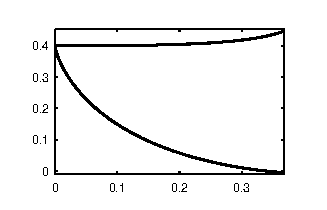
\includegraphics[width=6.5cm]{../EPS/Gamma_a2_p2} \hspace{5mm}
  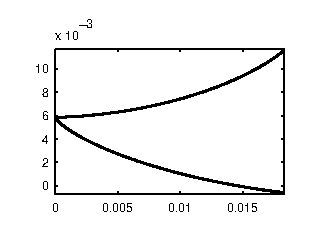
\includegraphics[width=6.5cm]{../EPS/Gamma_a5_p2}}
%
\begin{picture}(0,0)
\put(263,28){\footnotesize $\alpha = 2$}
\put(365,97){$\phi_0$}
\put(323,46){$\phi_{-1}$}
%
\put(470,28){\footnotesize $\alpha = 5$}
\put(545,93){$\phi_0$}
\put(570,35){$\phi_{-1}$}
%
\put(324,0){(a)}
\put(531,0){(b)}
\end{picture}
\end{figure}

\end{document}
